\documentclass[border=3pt]{standalone}
% Shared style for all figures: Latin Modern to match the manuscript, and the
% Okabe-Ito colour-blind-safe palette.
\usepackage{lmodern}
\usepackage[T1]{fontenc}
\usepackage{pgfplots}
\usepackage{pgfplotstable}
\pgfplotsset{compat=1.18}
\usetikzlibrary{positioning,arrows.meta,fit,calc,backgrounds,patterns}
\definecolor{oiblue}{HTML}{0072B2}
\definecolor{oiorange}{HTML}{E69F00}
\definecolor{oigreen}{HTML}{009E73}
\definecolor{oivermillion}{HTML}{D55E00}
\definecolor{oisky}{HTML}{56B4E9}
\definecolor{oipurple}{HTML}{CC79A7}
\definecolor{oigrey}{HTML}{999999}
\pgfplotsset{every axis/.append style={font=\small, tick label style={font=\footnotesize},
  label style={font=\small}, legend style={font=\footnotesize, draw=none}}}

\usepackage{amsmath}
\hyphenpenalty=10000
\newcommand{\Call}{\mathsf{Call}}
\newcommand{\ptext}{\mathsf{text}}
\newcommand{\pvar}{\mathsf{var}}
\newcommand{\pres}{\mathsf{res}}
\begin{document}
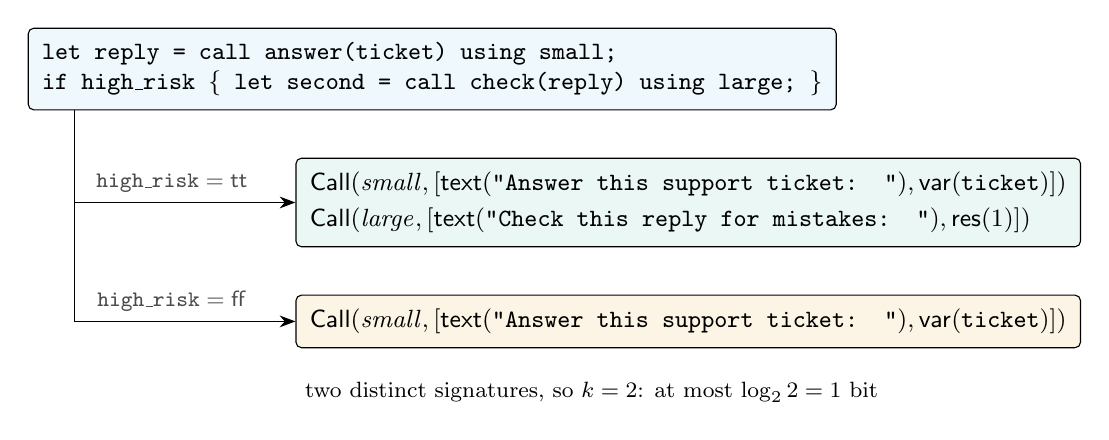
\begin{tikzpicture}[
    font=\small, >={Stealth[length=2mm]},
    box/.style={draw, rounded corners=2pt, align=left, inner sep=5pt, fill=white},
    head/.style={font=\small\bfseries, align=center},
    lab/.style={font=\footnotesize, text=black!70}]
  \node[box, fill=oisky!10, anchor=north west] (src) at (0,0) {%
    \texttt{let reply = call answer(ticket) using small;}\\
    \texttt{if high\_risk \{ let second = call check(reply) using large; \}}};
  \node[box, fill=oigreen!8, anchor=north west] (tt) at ([xshift=34mm, yshift=-6mm]src.south west) {%
    $\Call(\mathit{small}, [\ptext(\text{\texttt{"Answer this support ticket: "}}), \pvar(\texttt{ticket})])$\\[2pt]
    $\Call(\mathit{large}, [\ptext(\text{\texttt{"Check this reply for mistakes: "}}), \pres(1)])$};
  \node[box, fill=oiorange!10, anchor=north west] (ff) at ([yshift=-6mm]tt.south west) {%
    $\Call(\mathit{small}, [\ptext(\text{\texttt{"Answer this support ticket: "}}), \pvar(\texttt{ticket})])$};
  \coordinate (spine) at ([xshift=6mm]src.south west);
  \draw[->] (spine) |- node[lab, above, pos=0.72]{$\texttt{high\_risk} = \mathsf{tt}$} (tt.west);
  \draw[->] (spine) |- node[lab, above, pos=0.72]{$\texttt{high\_risk} = \mathsf{ff}$} (ff.west);
  \node[lab, text=black, anchor=north west] at ([yshift=-3mm]ff.south west) {two distinct signatures, so $k = 2$: at most $\log_2 2 = 1$ bit};
\end{tikzpicture}
\end{document}
